\subsubsection*{الف}
در این بخش فرض می‌کنیم هیچ وابستگی‌ای بین دستورات وجود ندارد.

\setLTR
$
SpeedUp = \frac{T_1}{T_2} = \frac{CPI_1\times\frac{1}{CR_1}}{CPI_2\times\frac{1}{CR_2}} = \frac{\frac{5}{2.5}}{\frac{1}{2}} = 4
$
\setRTL

اولین حلقه 4 کلاک نیاز دارد و حلقه‌های بعدی در 1 کلاک اجرا می‌شوند.

\subsubsection*{ب}

\setLTR
\qquad \qquad \qquad \qquad \qquad 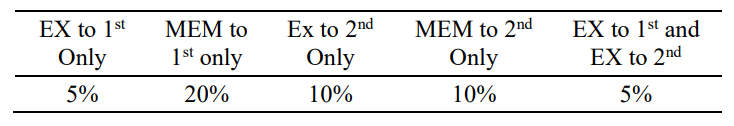
\includegraphics[width=0.5\linewidth]{figs/screenshot001}
\setRTL

فرض می‌کنیم درصد دستوراتی که وابستگی دارند مطابق جدول فوق است، پس برای هر نوع از دستورات تعداد چرخه تاخیر را محاسبه می‌کنیم	و سپس با فرض این که هیچ
$Forwarding$
ای نداریم، تسریع را حساب می‌کنیم:

\setLTR
$
\begin{cases}
	EX \ to \ 1st \ Only = 2 Delay Cycle \\
	MEM \ to \ 1st \ Only =2 Delay Cycle \\
	EX \ to \ 2nd \ Only = 1 Delay Cycle\\ 
	MEM \ to \ 2nd \ Only =1 Delay Cycle\\
	EX \ to \ 1st = 2 Delay Cycle\\
	EX \ to \ 2nd =  2 Delay Cycle
	\end{cases}
$

$
SpeedUp = \frac{T_1}{T_2} = \frac{\frac{CPI_1}{CR_1}}{\frac{CPI_2}{CR_2}} =
 \frac{\frac{5}{2.5}}{
\frac{0.05\times3 + 0.2\times3+0.1\times2+0.1\times2+0.05\times3+ 0.5\times1}{2}
} \simeq 2.2
$
\setRTL


\subsubsection*{ج}

اگر داده‌ها را به صورت زودهنگام در اختیار داشته باشیم باید فقط برای وابستگی 
$MEM \ to \ 1st \ only$
1 کلاک به تاخیر کنیم. پس:

\setLTR
$
SpeedUp = \frac{T_1}{T_2} = \frac{\frac{CPI_1}{CR_1}}{\frac{CPI_2}{CR_2}} = \frac{\frac{5}{2.5}}{\frac{0.2\times2 + 0.8\times1}{2}} = \frac{10}{3} 
\simeq 3.3
$
\setRTL

\subsubsection*{د}

در این صورت برای محاسبه شرط Branch باید یک چرخه Stall داشته باشیم. پس:

\setLTR
$
SpeedUp = \frac{T_1}{T_2} = \frac{\frac{CPI_1}{CR_1}}{\frac{CPI_2}{CR_2}} = \frac{\frac{5}{2.5}}{\frac{0.2\times2 + 0.1\times2+0.7\times1}{2}} \simeq 3.1
$
\setRTL

\pagebreak

\subsubsection*{ه}

اگر همه پرش‌ها را انجام نشده فرض کنیم، آن‌وقت تسریع برابر است با:

\setLTR
$
SpeedUp = \frac{T_1}{T_2} = \frac{\frac{CPI_1}{CR_1}}{\frac{CPI_2}{CR_2}} = \frac{5}{0.2\times2+0.1\times(0.2\times1+0.8\times2)+0.7\times1} \times \frac{2}{2} \simeq 3.12
$
\setRTL


